\documentclass[tikz]{standalone}
\usetikzlibrary{arrows,angles,quotes,calc,decorations.pathreplacing}
\begin{document}
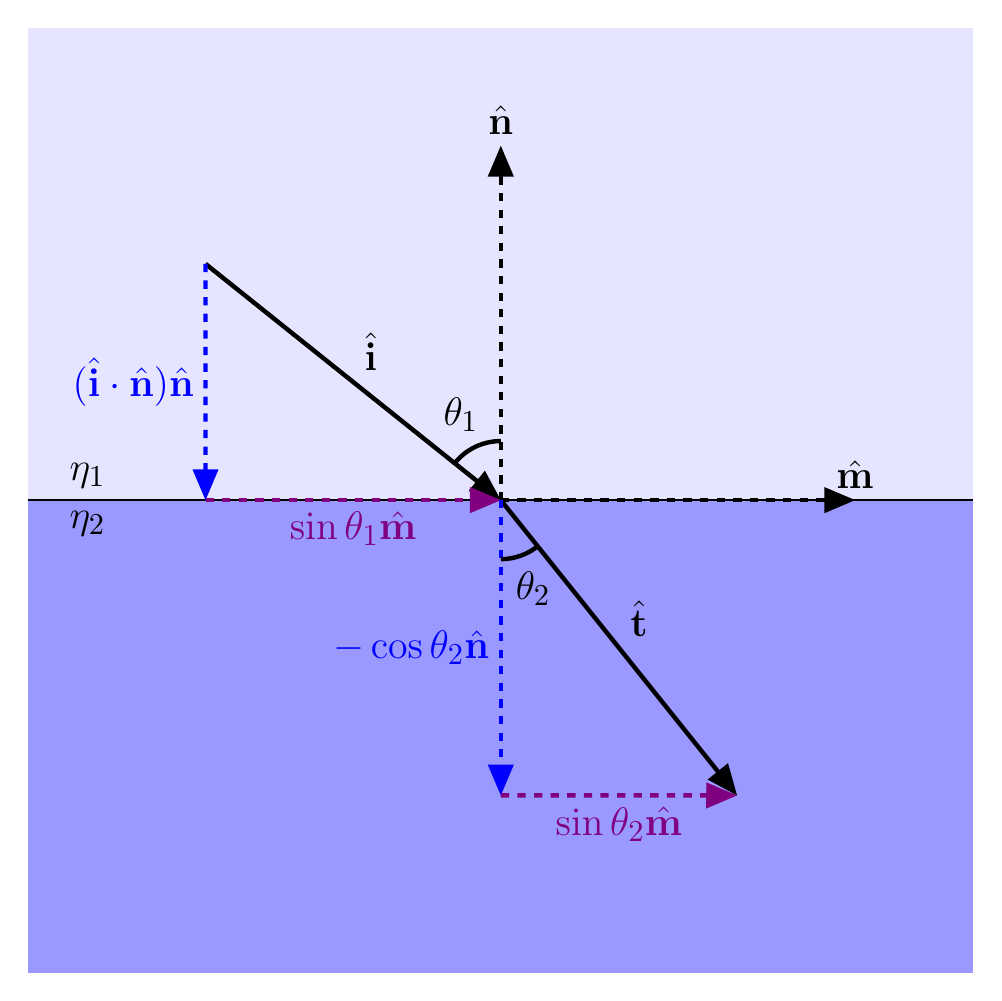
\begin{tikzpicture}[>=triangle 45,line width=1.6pt,scale=1.5,font=\fontsize{15pt}{0}]
  \coordinate (O) at (0,0);
  \coordinate (V) at (-2.5,2);
  \coordinate (R) at (2,-2.5);
  \coordinate (N)  at (0, 3);
  \coordinate (M)  at (3, 0);
  \fill[blue!10] (-4,0) rectangle (4,4);
  \fill[blue!40] (-4,0) rectangle (4,-4);
  \draw[line width=0.5pt] (-4, 0) -- (4, 0);
  \draw[->, style=dashed] (O) -- (N) node[anchor=south] {$\hat{\mathbf{n}}$};
  \draw[->, style=dashed] (O) -- (M) node[anchor=south] {$\hat{\mathbf{m}}$};
  \draw[->] (V) -- (O) node[midway, anchor=south west] {$\hat{\mathbf{i}}$};
  \draw[->] (O) -- (R) node[midway, anchor=south west] {$\hat{\mathbf{t}}$};
  \draw[->, blue, style=dashed] (V) -- (-2.5, 0) node[midway, anchor=east] {$(\hat{\mathbf{i}} \cdot \hat{\mathbf{n}})\hat{\mathbf{n}}$};
  \draw[->, violet, style=dashed] (-2.5, 0) -- (O) node[midway, anchor=north] {$\sin\theta_1\hat{\mathbf{m}}$};
  \draw[->, blue, style=dashed] (O) -- (0, -2.5) node[midway, anchor=east] {$-\cos\theta_2\hat{\mathbf{n}}$};
  \draw[->, violet, style=dashed] (0, -2.5) -- (R) node[midway, anchor=north] {$\sin\theta_2\hat{\mathbf{m}}$};
  \draw (0,0.5) arc (90:140:0.5);
  \draw (0,-0.5) arc (270:310:0.5);
  \node[] at (115:0.8)  {$\theta_{1}$};
  \node[] at (290:0.8)  {$\theta_{2}$};
  \node[anchor=south] at (-3.5, 0) {$\eta_1$};
  \node[anchor=north] at (-3.5, 0) {$\eta_2$};
\end{tikzpicture}
\end{document}
